\section{Iteration 7: Decomposition of the Outbound Communication Scheduler}
\label{add:it7}

\subsection{Step 1: Identify candidate drivers}
\label{add:it7/drivers}

\npar It is crucial that ``shut down valve" trames are sent in time to the
correct module considering that trames that arrive too late can ultimately
lead to a potential disaster claiming the lifes of several people. Therefore the
outbound trames (i.e. towards modules) need to be scheduled. 

\npar The (only) driver of this iteration is 

\begin{itemize}
  	\item P1': Timely closure of valves.
  	\begin{itemize}
  		\item Alarm trames have to be handled within a bounded time. 
    \end{itemize}
\end{itemize}

\npar No use cases were delegated to this scheduler.

\subsection{Step 2: Choose design concepts}
\label{add:it7/concepts}

\npar The design concepts for this decomposition are exactly the same as those
of the storage and anomaly detection scheduler, see sections
\ref{add:it3/concepts} and \ref{add:it5/concepts}.
This is a logical result considering that both schedulers are established with
performance drivers in mind.

\subsection{Step 3: Instantiate architectural elements and allocate responsibilities}
\label{add:it7/elements}

\begin{figure}[H]
	\begin{centering}
		% TODO Figure
		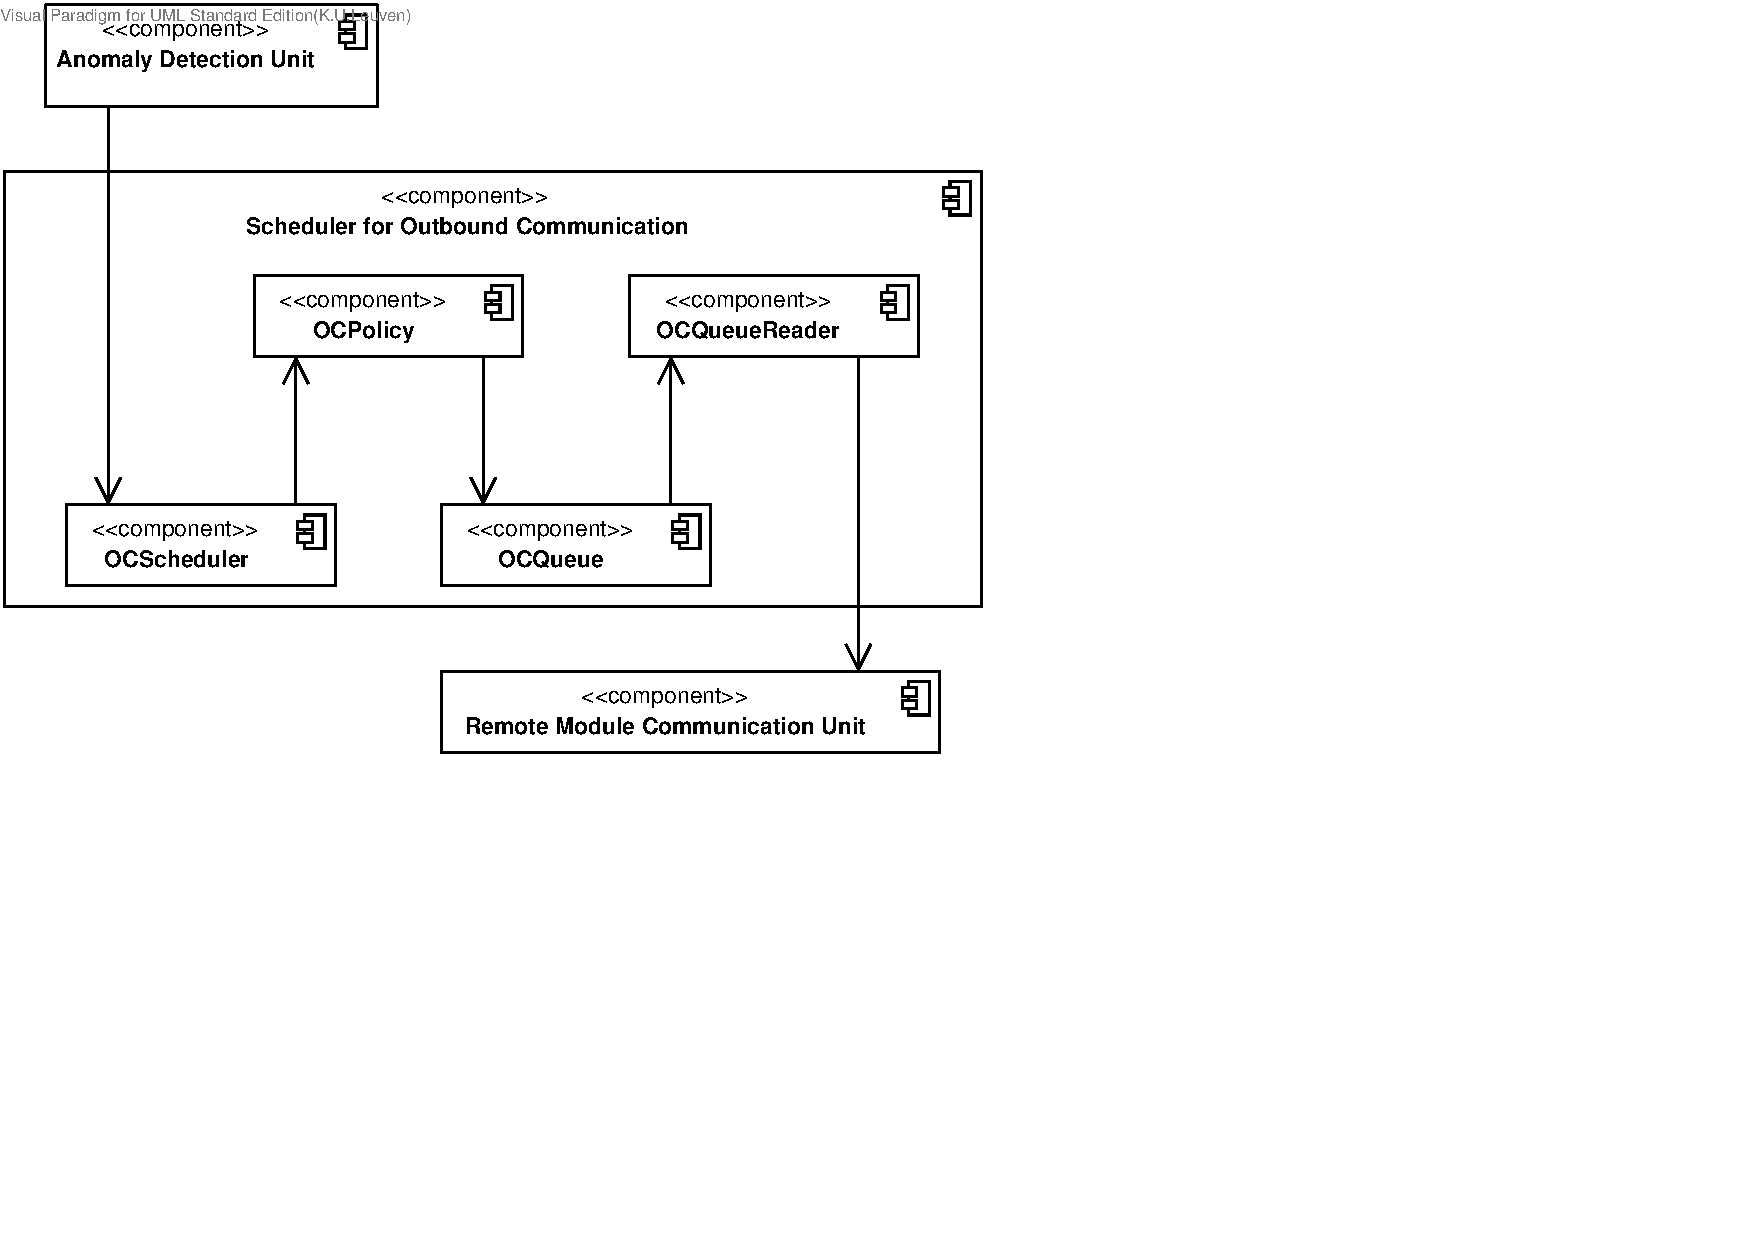
\includegraphics[width=\textwidth]{figs/add-it7-elements.pdf}
		\caption{Overview of the instantiated child elements in the Scheduler For
		Outbound Communication.}
		\label{fig:it7/elements}
	\end{centering}
\end{figure}

\subsubsection{OCScheduler}

\npar The OCScheduler serves as entry point for the OCCommand scheduling. Upon
receiving a command the scheduler will place that command in an
OCPolicy. When the system transitions between load modi (from normal
to overload or vice versa) it is possible to change the current policy.
This transition in policies is likewise the responsibility of this component.

\subsubsection{OCPolicy}

\npar An OCPolicy is responsible for inserting incoming OCCommands (received
from the OCScheduler) into the OCQueue. To be able to do this, the policy first
has to determine the priority of the incoming OCCommand (and this priority is
different for the various policies).

\subsubsection{OCQueue}

\npar The OCQueue does nothing else than provide a priority queue for
OCCommands with accompanying insert and retrieve functionality. Since
it is a priority queue the commands can be placed in different places in the
queue depending on their priority. More precisely, for each priority level will
the index of the last element with that priority be kept in a list. When a new
command needs to be inserted, the priority of that command is determined.
Subsequently, the priority is used to retrieve the index of the last element
(with the same priority) and in this way the new command can be inserted.

\subsubsection{OCQueueReader}

\npar The purpose of this component is dequeueing the OCQueue and
afterwards dispatch the popped command to the the Remote Module Communication
Unit.

% \npar The design of the outbound communication scheduler is analogous to that
% of the storage scheduler and the anomaly detection scheduler. This is rather
% locical because they all have the same purpose: schedule commands of some kind.
% 
% \npar All requests to the Outbound Communication Scheduler are encapsulated as
% OCCommand objects. These objects represent requests to send a certain control
% trame to a given remote device for some reason. 
% 
% \npar The scheduler (OCScheduler) handles every incoming command
% (OCCommand) by inserting the command in a queue (OCQueue) with a
% certain priority using a policy (OCPolicy). The scheduling policy
% determines the priority of the command based on the nature of that command
% (in particular, the reason for the request). As before, priorities of commands
% already in the queue are increased every time a new command is inserted.
% Again, this is done to prevent starvation.
% 
% \npar An additional component (OCQueueReader) will pop the command with the
% highest priority off the queue and present it on the database for execution.

\subsection{Step 4: Define interfaces for instantiated elements}
\label{add:it7/interfaces}

\npar In this section each interface is explained in terms of the components
which use and/or offer it together with information about what is exchanged. For
detailed information with reference to the specific methods the interfaces
implement, we refer to the interface catalog, see appendix
\ref{chap:interface-catalog}.

\subsubsection{OCSchedulerAPI}

\npar The \interface{OCSchedulerAPI} was already discussed in section
\ref{add:it1/interfaces}.

\subsubsection{OCPolicyAPI}

\npar The \interface{OCPolicyAPI} lies between the OCScheduler and the OCPolicy.
Its goal is to pass through commands which have to be placed in an OCQueue.

\subsubsection{OCQueueAPI}

\npar This interface is offered by the OCQueue and used by both the OCPolicy and
the OCQueueReader. The policy uses the interface to place commands in the queue
and the reader pops them off.

\begin{figure}[H]
	\begin{centering}
		% TODO Figure
		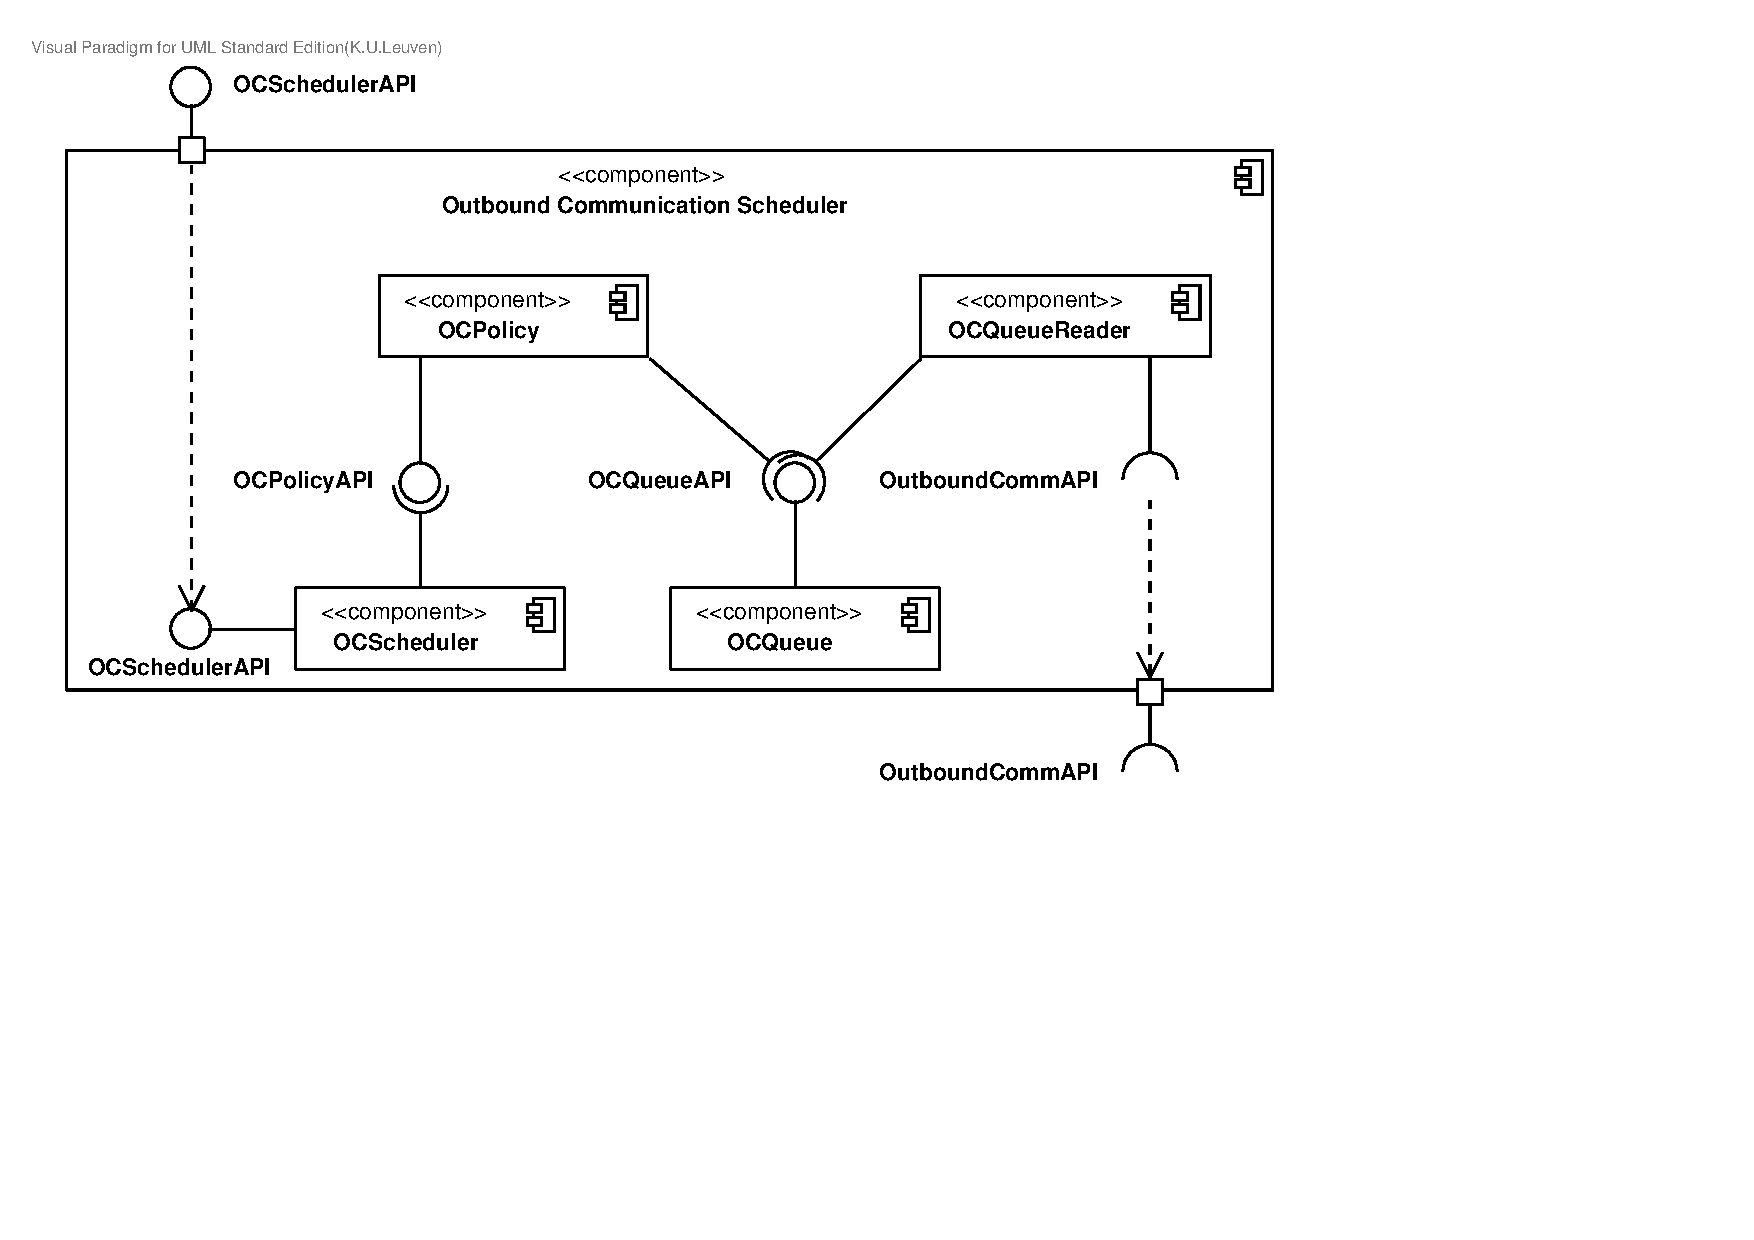
\includegraphics[width=\textwidth]{figs/add-it7-interfaces.pdf}
		\caption{Overview of the interfaces and components in the Scheduler For
		Outbound Communication.}
		\label{fig:it7/interfaces}
	\end{centering}
\end{figure}

\subsection{Step 5: Verify and refine}
\label{add:it7/verification}

\npar The driver for this iteration, P1, is resolved. The scheduler policy will
prioritize outbound messages that are intended to close valves after an anomaly
is detected.
